\documentclass[a4paper]{memoir}

\usepackage[utf8]{inputenc}
\usepackage[a4paper,margin=3cm]{geometry}
%\usepackage[symbol]{footmisc}
\renewcommand*{\thefootnote}{\fnsymbol{footnote}} % footnotes

\usepackage{booktabs}
\usepackage{caption}
\usepackage[labelformat=simple]{subcaption}
\usepackage{multirow}
\usepackage{geometry}

\usepackage{graphicx}
\usepackage[dvipsnames]{xcolor}
\usepackage{tikz}
\usepackage{pgfplots}
\usepackage{comment}

\usepackage{amsmath, amsfonts}
\usepackage{amssymb}
\usepackage{physics}

\usepackage{bm}
\usepackage{listings}

\usepackage{hyperref}
\hypersetup{
	colorlinks=true,
	urlcolor=tabblue,
	linkcolor=tabblue,
	citecolor=tabblue
}

\usepackage[citestyle=numeric-comp]{biblatex}

%%%%%%% TIKZ OPTIONS FOR PGFPLOTSX
\usetikzlibrary{arrows.meta}
\usetikzlibrary{backgrounds}
\usetikzlibrary{decorations.markings}
\usetikzlibrary{patterns}
\pgfplotsset{compat=newest}
\usepgfplotslibrary{patchplots}
\usepgfplotslibrary{fillbetween}
\pgfplotsset{%
    layers/standard/.define layer set={%
        background,axis background,axis grid,axis ticks,axis lines,axis tick labels,pre main,main,axis descriptions,axis foreground%
    }{
        grid style={/pgfplots/on layer=axis grid},%
        tick style={/pgfplots/on layer=axis ticks},%
        axis line style={/pgfplots/on layer=axis lines},%
        label style={/pgfplots/on layer=axis descriptions},%
        legend style={/pgfplots/on layer=axis descriptions},%
        title style={/pgfplots/on layer=axis descriptions},%
        colorbar style={/pgfplots/on layer=axis descriptions},%
        ticklabel style={/pgfplots/on layer=axis tick labels},%
        axis background@ style={/pgfplots/on layer=axis background},%
        3d box foreground style={/pgfplots/on layer=axis foreground},%
    },
}

\newcommand{\beq}{\begin{equation}}
\newcommand{\eeq}{\end{equation}}
\newcommand{\sgn}{\mathrm{sgn}}

\newcommand{\red}[1]{\color{red}{#1}}

\newcommand{\mref}{{\color{red}0.0}} % missing ref
\newcommand{\todo}{\noindent{\color{tabred}[To be continued\dots]}}

\definecolor{tabred}{RGB}{214, 39, 40}
\definecolor{tabblue}{HTML}{1f77b4}
\definecolor{tabgreen}{HTML}{2ca02c}

%\usepackage[usenames,dvipsnames]{color} % more flexible names for syntax highlighting colors

\lstset{
    basicstyle=\ttfamily, 
    numbers=left, 
    numberstyle=\small\ttfamily\color{ForestGreen},
    stepnumber=1,              
    numbersep=10pt, 
    numberfirstline=true, 
    numberblanklines=true, 
    tabsize=4,
    lineskip=0pt,
    aboveskip=10pt,
    belowskip=10pt,
    extendedchars=true,
    breaklines=true,
    %backgroundcolor=\color{ForestGreen!10},
    keywordstyle=\color{blue}\bfseries,
    identifierstyle=, % using emph or index keywords
    commentstyle=\color{ForestGreen},
    stringstyle=\color{Maroon},
    showstringspaces=false,
    showtabs=false,
    upquote=false,
    texcl=true % interpet comments as LaTeX
}

\lstdefinelanguage{julia}
{
  keywordsprefix=\@,
  morekeywords={
    exit,whos,edit,load,is,isa,isequal,typeof,tuple,ntuple,uid,hash,finalizer,convert,promote,
    subtype,typemin,typemax,realmin,realmax,sizeof,eps,promote_type,method_exists,applicable,
    invoke,dlopen,dlsym,system,error,throw,assert,new,Inf,Nan,pi,im,begin,while,for,in,return,
    break,continue,macro,quote,let,if,elseif,else,try,catch,end,bitstype,ccall,do,using,module,
    import,export,importall,baremodule,immutable,local,global,const,Bool,Int,Int8,Int16,Int32,
    Int64,Uint,Uint8,Uint16,Uint32,Uint64,Float32,Float64,Complex64,Complex128,Any,Nothing,None,MPO,MPS,
    function,type,typealias,abstract
  },
  sensitive=true,
  morecomment=[l]{\#},
  morestring=[b]',
  morestring=[b]" 
}

% Captions

\newcommand*{\CaptionVLineWidth}{0.5pt}
\newcommand*{\CaptionVLineSep}{.5em}

\newcommand*{\CaptionVLine}{%
	\noindent
	\kern\dimexpr-\CaptionVLineSep-\CaptionVLineWidth\relax
	\textcolor{tabblue}{\vline width\CaptionVLineWidth}%
	\kern\CaptionVLineSep\relax
}

\DeclareCaptionFormat{vLine}[%
#1#2\CaptionVLine#3\par % Single line captions
]{% Multi-line captions
	\caption@ifin@list\caption@lsepcrlist\caption@lsepname{%
		\caption@Error{%
			The option `labelsep=\caption@lsepname' does not work\MessageBreak
			with `format=hang'}
	}{%
		\sbox0{%
			\parbox[t]{\linewidth}{%
				\@hangfrom{#1#2}%
				\advance\caption@parindent\hangindent
				\advance\caption@hangindent\hangindent
				\xdef\CaptionHangIndent{\the\hangindent}%
				\caption@@par#3\par
			}%
		}%
		\noindent
		\kern\CaptionHangIndent\relax
		\CaptionVLine
		\kern-\CaptionHangIndent\relax
		\usebox0%
	}%
}

\captionsetup{
	labelsep=quad,
	labelfont={color=tabblue},
	format=vLine,
}
\captionsetup[sub]{
	labelsep=quad,
}
\addbibresource{misc/bibliography.bib}

\begin{document}
	
\pagenumbering{gobble}

\begin{center}
    {\bfseries {\Large Numerical analysis of superconducting phases in the}} \\[0.8em]
    {\bfseries {\Large extended Hubbard model with non-local pairing}} \\[1em]
    \large University of Pisa, a.y.~2025-2026 \\[0.8em]
    Alessandro Gori\footnote{\href{mailto:a.gori23@studenti.unipi.it}{a.gori23@studenti.unipi.it} / \href{https://github.com/nepero27178}{nepero27178@github.com}} \\[0.8em]
    \scriptsize Thesis for the Master's degree in Physics
    
\end{center}

\renewcommand*{\thefootnote}{\arabic{footnote}}
\setcounter{footnote}{0}

\begin{abstract}
    \todo
\end{abstract}

% Enable if class: memoir
\begin{KeepFromToc}		% No ToC entry in ToC
	\tableofcontents
\end{KeepFromToc}

\vfill
\begin{flushright}
	\textit{Draft: \today}
\end{flushright}
\clearpage

\newgeometry{
	left=2.5cm,
	right=2.5cm}
	\thispagestyle{plain}
	\begin{table}
		\centering
		\begin{tabular}{r c}
			\multicolumn{2}{c}{\textbf{List of symbols and abbreviations}} \\
			\midrule
			$\mathrm{AF}$ & Anti-Ferromagnetic \\
			$\mathrm{SC}$ & Superconductor \\
			$\mathrm{T}_c$ & Critical temperature \\
		\end{tabular}
	\end{table}
\restoregeometry 
	% Uncomment
%\clearpage					% Uncomment
%\isopage[12]
%\checkandfixthelayout

% Front matter
\pagestyle{plain}

\chapter*{Introduction}
This thesis project is about my favorite ice cream flavor. \todo	% Uncomment

% Main matter
\pagenumbering{arabic}
% \lipsum[1-10]

\let\oldmarginpar\marginpar
\renewcommand{\marginpar}[1]{
	\oldmarginpar{
		\small
		\textit{{#1}}
	}
}
\lipsum[11]\marginpar{Lipsum 11}

\lipsum[12-15]

\epigraph{If you try and take a cat apart to see how it works, the first thing you have on your hands is a nonworking cat.}{Douglas Adams} % Test chapter
\chapter{Theoretical introduction}\label{chapter:theoretical-introduction}

\todo

\section{Antiferromagnetic ordering in the Hubbard model}

Consider the ordinary Hubbard model:
\begin{equation}\label{eq:hubbard-model}
	\hat H = 
	-t \sum_{\langle ij \rangle} \sum_\sigma \hat c_{i\sigma}^\dagger \hat c_{j\sigma}
	+ U \sum_i \hat n_{i\uparrow} \hat n_{i\downarrow}
	\qquad
	t, U  > 0
\end{equation}
The two competing mechanisms are site-hopping of amplitude $t$ and local repulsion of amplitude $U$. For this model defined \textbf{on a bipartite lattice at half filling} and fixed electron number, it is well known \mref{} that below a certain critical temperature $T_c$ the ground-state acquires antiferromagnetic ($\mathrm{AF}$) long-range ordering. schematically depicted in Fig.~\ref{fig:antiferromagnet}. The mechanism for the formation of the $\mathrm{AF}$ phase takes advantage of virtual hopping, as described in App.~\ref{appendix:superexchange-virtual-hopping}.

\begin{figure}
	\centering
	\newcount\xLength
\xLength=4	% Even!
\newcount\yLength
\yLength=2	% Even!

\newcount\xStop
\xStop=\xLength
\divide\xStop by 2 \advance\xStop by -1\relax

\newcount\yStop
\yStop=\yLength
\divide\yStop by 2 \advance\yStop by -1\relax

\def\angle{60}
\def\arrowLength{0.5}

\begin{tikzpicture}
	\draw[
		color=lightgray, dashed
	] 
		(-0.25,-0.25) grid ({\xLength+0.25}, {\yLength+0.25});
		
	% Nested, no indentation
	\foreach \x in {
		0,...,\xStop
	}{
	\foreach \y in {
		0,...,\yStop
	}{
		% Up sites
		\fill[color=tabred] 
			({2*\x},{2*\y}) circle (1.5pt)
			({2*\x+1},{2*\y+1}) circle (1.5pt)
		;
		
		% Up arrows
		\draw[color=tabred, -stealth]
			(
				{2*\x - \arrowLength/2 * cos(\angle)},
				{2*\y - \arrowLength/2 * sin(\angle)}
			) --++ (
				{\arrowLength * cos(\angle)},
				{\arrowLength * sin(\angle)}
			);
		\draw[color=tabred, -stealth]
			(
				{2*\x+1 - \arrowLength/2 * cos(\angle)},
				{2*\y+1 - \arrowLength/2 * sin(\angle)}
			) --++ (
				{\arrowLength * cos(\angle)},
				{\arrowLength * sin(\angle)}
			);
		
		% Down sites
		\fill[color=tabblue] 
			({2*\x},{2*\y+1}) circle (1.5pt)
			({2*\x+1},{2*\y}) circle (1.5pt)
		;
		
		% Down arrows
		\draw[color=tabblue, stealth-]
			(
				{2*\x+1 - \arrowLength/2 * cos(\angle)},
				{2*\y - \arrowLength/2 * sin(\angle)}
			) --++ (
				{\arrowLength * cos(\angle)},
				{\arrowLength * sin(\angle)}
			);
		\draw[color=tabblue, stealth-]
			(
				{2*\x - \arrowLength/2 * cos(\angle)},
				{2*\y+1 - \arrowLength/2 * sin(\angle)}
			) --++ (
				{\arrowLength * cos(\angle)},
				{\arrowLength * sin(\angle)}
			);
	}}

	% Border
	\foreach \x in {
		0, ..., \xStop
	}{
	\foreach \y in {
		0, ..., \yStop
	}{
	
		% Up sites
		\fill[color=tabred] 
			({2*\x},\yLength) circle (1.5pt)
			(\xLength,{2*\y}) circle (1.5pt)
		;
		
		% Up arrows
		\draw[color=tabred, -stealth]
			(
				{2*\x - \arrowLength/2 * cos(\angle)},
				{\yLength - \arrowLength/2 * sin(\angle)}
			) --++ (
				{\arrowLength * cos(\angle)},
				{\arrowLength * sin(\angle)}
			);
		\draw[color=tabred, -stealth]
			(
				{\xLength - \arrowLength/2 * cos(\angle)},
				{2*\y - \arrowLength/2 * sin(\angle)}
			) --++ (
				{\arrowLength * cos(\angle)},
				{\arrowLength * sin(\angle)}
			);
		
		% Down sites
		\fill[color=tabblue] 
			({2*\x+1},\yLength) circle (1.5pt)
			(\xLength,{2*\y+1}) circle (1.5pt)
		;
		
		% Down arrows
		\draw[color=tabblue, stealth-]
			(
				{2*\x+1 - \arrowLength/2 * cos(\angle)},
				{\yLength - \arrowLength/2 * sin(\angle)}
			) --++ (
				{\arrowLength * cos(\angle)},
				{\arrowLength * sin(\angle)}
			);
		\draw[color=tabblue, stealth-]
			(
				{\xLength - \arrowLength/2 * cos(\angle)},
				{2*\y+1 - \arrowLength/2 * sin(\angle)}
			) --++ (
				{\arrowLength * cos(\angle)},
				{\arrowLength * sin(\angle)}
			);
	}}

	% Topright
	\fill[color=tabred] 
		(\xLength,\yLength) circle (1.5pt);
	\draw[color=tabred, -stealth]
		(
			{\xLength - \arrowLength/2 * cos(\angle)},
			{\yLength - \arrowLength/2 * sin(\angle)}
		) --++ (
			{\arrowLength * cos(\angle)},
			{\arrowLength * sin(\angle)}
		);
		
\end{tikzpicture}
	\caption{Schematic representation of the \AF phase.}
	\label{fig:antiferromagnet}
\end{figure}

App.~\ref{appendix:mean-field-hubbard} describes the Mean-Field Theory description of ferromagnetic-antiferromagnetic orderings in $2\mathrm{D}$ Hubbard lattices.

\section{The Extended Fermi-Hubbard model}

The Extended Fermi-Hubbard model is defined by:
\begin{equation}\label{eq:extended-hubbard-model}
	\hat H = 
	-t \sum_{\langle ij \rangle} \sum_\sigma \hat c_{i\sigma}^\dagger \hat c_{j\sigma}
	+ U \sum_i \hat n_{i\uparrow} \hat n_{i\downarrow}
	- V \sum_{\langle ij \rangle} \sum_{\sigma \sigma'} \hat n_{i\sigma} \hat n_{j\sigma'}
\end{equation}
The last term represents an effective attraction between neighboring electrons, of amplitude $V$. Such an interaction is believed \cite{cao2025p-wave} to be a necessary ingredient to describe the insurgence of high-$T_c$ superconductivity in cuprate SCs. \todo

{\color{tabred}
\begin{enumerate}
	\item Fourier transform and Brillouin zone;
	\item Pairing operator;
\end{enumerate}}

% Back matter
\appendix
%\chapter{Superexchange and virtual hopping in Hubbard lattices}\label{appendix:superexchange-virtual-hopping}

A key mechanism in \AF phase formation in Hubbard lattice is superexchange. The \AF phase is stabilized by spin fluctuations and second-order virtual hopping. The mechanism becomes clear enough by considering a $2$-sites Hubbard toy model.

\section{Virtual hopping in the $2$-sites Hubbard lattice}

\begin{figure}
	\centering
	\def\xSeparation{2}			% Lattice spacing
\def\ySeparation{1.5}		% Rows spacing
\def\angle{90}				% Arrows angle (0 is horizontal)
\def\arrowLength{0.5}		% Arrows length
\def\onSiteSeparation{0.1}  % Arrows horizontal separation on site
\begin{tikzpicture}
	
	% Lattice
	\foreach \i in {0,1,2}{
		\filldraw[color=lightgray, fill=lightgray] 
			(0,{\i*\ySeparation}) circle (1.5pt) 
			--++ 
			({\xSeparation},0) circle (1.5pt);
	}
	
	% Local repulsion
	\node[anchor=west, align=left, xshift=1cm]
		at (
			{0 + \xSeparation},
			{0 + 2 * \ySeparation}
		) {Local repulsion};
	
	\fill[color=tabred!80, path fading=fade out]
		(
			{0},
			{2 * \ySeparation}
		) circle (10pt) node (LocRep) {};
	% Label must be defined outside not to conflict with path fading
	
	\node[color=tabred, anchor=east, xshift=-0.25cm]
		at (LocRep) {\small $U$};
	
	\draw[color=tabblue, -stealth]
		(
			{0 - \onSiteSeparation/2 - \arrowLength/2 * cos(\angle)},
			{0 + 2 * \ySeparation - \arrowLength/2 * sin(\angle)}
		) --++ (
			{\arrowLength * cos(\angle)},
			{\arrowLength * sin(\angle)}
		);
	\draw[color=tabblue, stealth-]
		(
			{0 + \onSiteSeparation/2 - \arrowLength/2 * cos(\angle)},
			{0 + 2 * \ySeparation - \arrowLength/2 * sin(\angle)}
		) --++ (
			{\arrowLength * cos(\angle)},
			{\arrowLength * sin(\angle)}
		);
	
	% Single hop
	\node[anchor=west, align=left, xshift=1cm]
		at (
			{0 + \xSeparation},
			{0 + \ySeparation}
		) {Single hop};
	\draw[color=tabblue, -stealth]
		(
			{0 - \arrowLength/2 * cos(\angle)},
			{0 + \ySeparation - \arrowLength/2 * sin(\angle)}
		) --++ (
			{\arrowLength * cos(\angle)},
			{\arrowLength * sin(\angle)}
		);
	
	\draw[color=tabgreen, dashed] 
		(
			{0 + \arrowLength/2 * cos(\angle)},
			{\ySeparation}
		) edge [-stealth, bend left=30]
			node[midway, anchor=south]
				{\small $-t$}
		(
			{0 + \xSeparation + \arrowLength/2 * cos(\angle)},
			{\ySeparation}
		);
	
	% Double hop
	\node[anchor=west, align=left, xshift=1cm]
		at (
			{0 + \xSeparation},
			{0}
		) {Double hop};
	\draw[color=tabblue, -stealth]
		(
			{0 - \arrowLength/2 * cos(\angle)},
			{0 - \arrowLength/2 * sin(\angle)}
		) --++ (
			{\arrowLength * cos(\angle)},
			{\arrowLength * sin(\angle)}
		);
	\draw[color=tabblue, stealth-]
		(
			{0 + \xSeparation - \arrowLength/2 * cos(\angle)},
			{0 - \arrowLength/2 * sin(\angle)}
		) --++ (
			{\arrowLength * cos(\angle)},
			{\arrowLength * sin(\angle)}
		);
		
	\draw[color=tabgreen, dashed] 
		(
			{0 + \arrowLength/2 * cos(\angle)},
			{0 + \arrowLength/2 * sin(\angle)}
		) edge [-stealth, bend left=30]
			node[midway, anchor=south]
				{\small $-t$}
		(
			{0 + \xSeparation + \arrowLength/2 * cos(\angle)},
			{0 + \arrowLength/2 * sin(\angle)}
		)
		(
			{0 - \arrowLength/2 * cos(\angle)},
			{0 - \arrowLength/2 * sin(\angle)}
		) edge [stealth-, bend right=30]
			node[midway, anchor=north]
				{\small $-t$}
		(
			{0 + \xSeparation - \arrowLength/2 * cos(\angle)},
			{0 - \arrowLength/2 * sin(\angle)}
		);
\end{tikzpicture}
	\caption{Two sites Hubbard model.}
	\label{appfig:two-sites-hubbard-model}
\end{figure}

Consider the toy model:
\[
	\hat H = 
	-t \left\lbrace \hat c_{1\uparrow}^\dagger \hat c_{2\uparrow} + \hat c_{1\downarrow}^\dagger \hat c_{2\downarrow} + \mathrm{h}.\mathrm{c}. \right\rbrace
	+ U \left\lbrace \hat n_{1\uparrow} \hat n_{1\downarrow} + \hat n_{2\uparrow} \hat n_{2\downarrow} \right\rbrace
\]
with $i=1,2$ the site index. The two sites are represented in Fig.~\ref{appfig:two-sites-hubbard-model}. The two competing processes are: 
\begin{enumerate}
	\item electrons inter-sites hopping with amplitude $-t$;
	\item local repulsion $+U$, acting when two anti-aligned electrons reside on the same site; 
\end{enumerate}

For an half-filled system, the Hilbert space is six-dimensional. I use the notation $\ket{n_{1\uparrow} n_{1\downarrow} n_{2\uparrow} n_{2\downarrow}}$ to indicate the six computational basis states:
\[
\begin{aligned}
	\ket{\psi_1} &\equiv \ket{1010} \\
	\ket{\psi_2} &\equiv \ket{1100} \\
\end{aligned}
\qquad
\begin{aligned}
	\ket{\psi_3} &\equiv \ket{1001} \\
	\ket{\psi_4} &\equiv \ket{0110} \\
\end{aligned}
\qquad
\begin{aligned}
	\ket{\psi_5} &\equiv \ket{0011} \\
	\ket{\psi_6} &\equiv \ket{0101} \\
\end{aligned}
\]
For example, the top panel of Fig.~\ref{appfig:two-sites-hubbard-model} shows state $\ket{\psi_2}$. 

\subsection{Exact solution of the half-filled model}

The hamiltonian matrix is directly evaluated in this basis
\[
	H_{ij} = \bra{\psi_i}{\hat H}\ket{\psi_j}
	\quad\implies\quad
	H = \begin{bmatrix}
		0 &    &    &    &    &    \\
		&  U & -t & -t &    &    \\
		& -t &    &    & -t &    \\
		& -t &    &    & -t &    \\
		&    & -t & -t &  U &    \\
		&    &    &    &    &  0 \\  
	\end{bmatrix}
\]
Empty slots in the matrix stand for zeros. Evidently the states $\ket{\psi_1}$ (both up) and $\ket{\psi_6}$ (both down) are zero-energy eigenstates. These states cannot realize electrons hopping because of Pauli principle. The internal $4 \times 4$ matrix is readily diagonalized by the means of a change of basis $V$,
\[
	V \begin{bmatrix}
		 U & -t & -t &     \\
		-t &    &    & -t  \\
		-t &    &    & -t  \\
		   & -t & -t &  U  \\
	\end{bmatrix} V^\dagger = \begin{bmatrix}
	E^- &   & 	& 	 \\
	    & 0 & 	&	 \\
		&   & U & 	 \\
		&	&	& E^+
	\end{bmatrix}
\]

\begin{table}
	\centering
	\begin{tabular}{c c c}
		Structure & Eigenstate & Energy \\
		\midrule
		Spin-$1/2$ singlet & $\displaystyle \frac{\ket{\phi_3} - \ket{\phi_4}}{\sqrt{2}}$ & $\displaystyle E^- = \frac{U}{2} - \sqrt{\frac{U^2}{4} + 4t^2}$ \\
		&&\\ % Extra space
		Spin-$1/2$ triplet & $\ket{\phi_1}, \displaystyle \frac{\ket{\phi_3} + \ket{\phi_4}}{\sqrt{2}}, \ket{\phi_6}$ & 0 \\
		&&\\ % Extra space
		&$\displaystyle \frac{\ket{\phi_2}-\ket{\phi_5}}{\sqrt{2}}$ & $U$\\
		&&\\ % Extra space
		&$\displaystyle \frac{\ket{\phi_2}+\ket{\phi_5}}{\sqrt{2}}$ & $\displaystyle E^+ = \frac{U}{2} + \sqrt{\frac{U^2}{4} + 4t^2}$ \\
	\end{tabular}
	\caption{List of exact eigenstates and relative energies for the $2$-sites half-filled Hubbard model.}
	\label{apptab:two-sites-hubbard-model-eigenstates}
\end{table}

Tab.~\ref{apptab:two-sites-hubbard-model-eigenstates} shows the eigenvectors and relative eigenvalues obtained from diagonalization. The ground-state is the singlet state,
\[
	\frac{\ket{\phi_3} - \ket{\phi_4}}{\sqrt{2}} = \frac{\ket{1010} - \ket{0101}}{\sqrt{2}} = \frac{\ket{\uparrow\downarrow} - \ket{\downarrow\uparrow}}{\sqrt{2}}
\]
of energy
\[
	E^- = \frac{U}{2} - \sqrt{\frac{U^2}{4} + 4t^2} \simeq - \frac{4t^2}{U}
\]
the latter equality being true if $U \gg t$ (strong repulsion limit). The singlet state pairs with a spatially-symmetric (nodeless) wavefunction. The entire triplet (second row of Tab.~\ref{apptab:two-sites-hubbard-model-eigenstates}) remains at zero energy. Excited states are anti-symmetrized and symmetrized version of the polarized states $\ket{\phi_1}$ and $\ket{\phi_6}$.

\subsection{Virtual hopping}

The key feature of the singlet state is the one represented in the bottom panel of Fig.~\ref{appfig:two-sites-hubbard-model}: if the two electrons occupy separate sites and are anti-aligned, both ``see'' the other site as empty, thus free to hop to. \todo
%\chapter{Mean-Field Theory in Hubbard lattices}\label{appendix:mean-field-hubbard}

In this Appendix the Mean-Field solutions to the Hubbard hamiltonian,
\[
	\hat H = 
	-t \sum_{\langle ij \rangle} \sum_\sigma \hat c_{i\sigma}^\dagger \hat c_{j\sigma}
	+ U \sum_i \hat n_{i\uparrow} \hat n_{i\downarrow}
	\qquad
	t, U  > 0
\]
are described. The discussion is limited to the two-dimensional square lattice. The two-dimensional square lattice extension of the two-sites model can be studied by the means of Mean Field Theory. We have:
\[
\begin{aligned}
	\hat n_{i\uparrow} \hat n_{i\downarrow} &= \left( \ev{\hat n_{i\uparrow}} + \delta \hat n_{i\uparrow} \right) \left( \ev{\hat n_{i\downarrow}} + \delta \hat n_{i\downarrow} \right) \\
	&\simeq \ev{\hat n_{i\uparrow}} \ev{\hat n_{i\downarrow}} +  \delta \hat n_{i\uparrow} \ev{\hat n_{i\downarrow}} + \ev{\hat n_{i\uparrow}} \delta \hat n_{i\downarrow} + \mathcal{O} \left(\delta n^2\right) \\
	&= - \ev{\hat n_{i\uparrow}} \ev{\hat n_{i\downarrow}} + \hat n_{i\uparrow} \ev{\hat n_{i\downarrow}} + \ev{\hat n_{i\uparrow}} \hat n_{i\downarrow} + \mathcal{O} \left(\delta n^2\right)
\end{aligned}
\]
where $\delta \hat n_{i\sigma} \equiv \hat n_{i\sigma} - \ev{\hat n_{i\sigma}}$ and orders higher than first have been ignored, assuming negligible fluctuations around the equilibrium single-site population. The first term of the above three can be neglected at fixed particles number, being a pure energy shift. 

\section{Ferromagnetic solution}

The Mean-Field Theory ferromagnetic solution prescribes an uniformly magnetized lattice,
\[
	\ev{\hat n_{i\uparrow}} = n+m
	\qquad
	\ev{\hat n_{i\downarrow}} = n-m
\]
where $n$ is the site electron density and $m$ is the density unbalance, leading to a magnetization per site $2m$. The mean-field hamiltonian with these substitutions becomes:
\[
\begin{aligned}
	\hat H &\simeq 
	-t \sum_{\langle ij \rangle} \sum_\sigma \hat c_{i\sigma}^\dagger \hat c_{j\sigma}
	+ U \sum_i \left[
		\hat n_{i\uparrow} \ev{\hat n_{i\downarrow}} + \ev{\hat n_{i\uparrow}} \hat n_{i\downarrow} 
	\right] \\
	&= -t \sum_{\langle ij \rangle} \sum_\sigma \hat c_{i\sigma}^\dagger \hat c_{j\sigma}
	+ nU \sum_i \left[
		\hat n_{i\uparrow} + \hat n_{i\downarrow} 
	\right] + mU \sum_i \left[
		\hat n_{i\uparrow} - \hat n_{i\downarrow} 
	\right]
\end{aligned}
\]
Fourier transforming,
\[
\begin{aligned}
	-t \sum_{\langle ij \rangle} \sum_\sigma \hat c_{i\sigma}^\dagger \hat c_{j\sigma} &= -2t \sum_{\mathbf{k}\sigma} \left[
		\cos(k_x) + \cos(k_y)
	\right] \hat n_{\mathbf{k}\sigma} \\
	nU \sum_i \left[
		\hat n_{i\uparrow} + \hat n_{i\downarrow} 
	\right] &= nU \sum_{\mathbf{k}\sigma} \hat n_{\mathbf{k}\sigma} \\
	mU \sum_i \left[
		\hat n_{i\uparrow} - \hat n_{i\downarrow} 
	\right] &= mU \sum_{\mathbf{k}\sigma} \left[
		\hat n_{\mathbf{k}\uparrow} - \hat n_{\mathbf{k}\downarrow}
	\right]
\end{aligned}
\]
having used adimensional lattice momenta. For a square lattice, the Brillouin Zone is delimited by
\[
	\mathbf{k} \in [-\pi,\pi] \times [-\pi,\pi]
\]
The hopping single-state energy is given by
\[
	\epsilon_{\mathbf{k}}^{(0)} = -2t \left[
		\cos(k_x) + \cos(k_y)
	\right]
\]
represented as a band in Fig.~\ref{appfig:ferromagnetic-3d-band}. At $U=0$, the mean-field ferromagnetic state fills the band bottom-up. The single-state energy becomes:
\[
\begin{aligned}
	\epsilon_{\mathbf{k}\uparrow} &= U \left(
		n+m
	\right) - 2t \left[
		\cos(k_x) + \cos(k_y)
	\right] \\
	\epsilon_{\mathbf{k}\downarrow} &= U \left(
		n-m
	\right) - 2t \left[
		\cos(k_x) + \cos(k_y)
	\right]
\end{aligned}
\]
Now it is a matter of finding the optimal value for $m$, minimizing the total energy at fixed filling $\rho = 2n$. Notice that said minimization is performed parametrically varying the magnetization $m$, inside the ferromagnetic-polarized space. As it turns out, for strong local repulsion $U/t \gg 1$, antiferromagnetic ordering is preferred. Comparison is needed in order to assess which magnetic ordering is preferred.

Consider the half-filling situation. An unpolarized system will have $n=1/4$, $m=0$: this implies $\ev{\hat n_{i\uparrow}} = \ev{\hat n_{i\downarrow}} = 1/4$. A perfectly up-ferromagnetic system, $n=1/4$, $m=1/4$: then $\ev{\hat n_{i\uparrow}} = 1/2$ and $\ev{\hat n_{i\downarrow}} = 0$. \todo

\begin{figure}
	\centering
	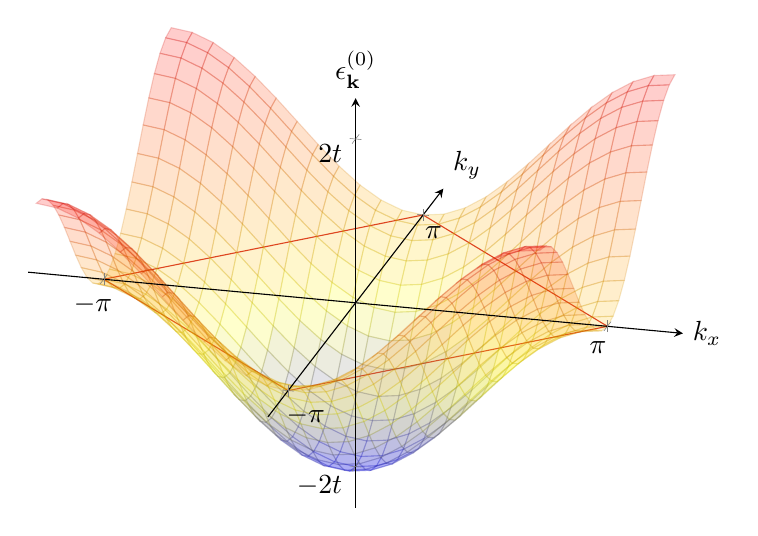
\begin{tikzpicture}
	\begin{axis}[
			axis on top,
			axis lines=center,
			xmin=-1.3, xmax=1.3,
			ymin=-1.3, ymax=1.3,
			zmin=-2.5, zmax=2.5,
			xtick={-1,1},
			ytick={-1,1},
			ztick={-2,2},
			xticklabels={$-\pi$,$\pi$},
			yticklabels={$-\pi$,$\pi$},
			zticklabels={$-2t$,$2t$},
			xlabel={$k_x$},
			ylabel={$k_y$},
			zlabel={$\epsilon_{\mathbf{k}}^{(0)}$},
			xlabel style={anchor=west},
			ylabel style={anchor=south west},
			zlabel style={anchor=south},
			width=\textwidth,
			view/az=15,
			view/el=30
		]
		\addplot3[
			domain=-1:0,
			color=tabred,
			dashed,
		]
		(
			{x},
			{-1-x},
			{0}
		);
		\addplot3[
			domain=0:1,
			color=tabred,
			dashed,
		]
		(
			{x},
			{-1+x},
			{0}
		);
		\addplot3[
			domain=-1:0,
			color=tabred,
			dashed,
		]
		(
			{x},
			{1+x},
			{0}
		);
		\addplot3[
			domain=0:1,
			color=tabred,
			dashed,
		]
		(
			{x},
			{1-x},
			{0}
		);
		
		\addplot3[
			domain=-1:1,
			samples=25,
			smooth,
			surf,
			opacity=0.2
		] { -cos(deg(pi*x))-cos(deg(pi*y)) };
		
		
	\end{axis}
\end{tikzpicture}
	\caption{Depiction of the Hubbard square lattice hopping band $\epsilon_{\mathbf{k}}^{(0)} = -2t[\cos(k_x) + \cos(k_y)]$. The red lines mark the zero-energy intersection.}
	\label{appfig:ferromagnetic-3d-band}
\end{figure}

{\color{tabred} Unclear: numerically, it turns out the paramagnetic phase ($m=0$) is preferred. Let $\Delta \equiv Um$ and ignore the constant contribution to energies $Un$: graphically, the $\uparrow$ band is shifted by $\Delta$, the $\downarrow$ band by $-\Delta$. At half-filling the Fermi energy remains fixed. For each quadrant (top view of the bands), the DoS is inversion-symmetric with respect to the anti-diagonal (red lines in Fig.~\ref{appfig:ferromagnetic-3d-band}), thus filling the bands bottom-up while performing the shifts should leave the total energy unchanged. Why is $m=0$ preferred?}

\section{Antiferromagnetic solution}

Consider now an AF mean-field solution. Let me change notation for a brief moment, indicating each site as
\[
	i \to \mathbf{r} = (x,y)
	\qquad
	x,y \in \mathbb{N}
\]
The mean-field AF solution at half-filling is the uniform-modulated magnetization
\[
	m_\mathbf{r} = (-1)^{x+y} m
	\qquad
	m \in [-1,1]
\]
and a mean-field Ansatz
\[
	\ev{\hat n_{\mathbf{r}\uparrow}} = n+m_\mathbf{r}
	\qquad
	\ev{\hat n_{\mathbf{r}\downarrow}} = n-m_\mathbf{r}
\]
With respect to the solution presented above, the only detail changing is the last term,
\[
	\hat H = -t \sum_{\langle \mathbf{r}\mathbf{r}' \rangle} \sum_\sigma \hat c_{\mathbf{r}\sigma}^\dagger \hat c_{\mathbf{r}'\sigma}
	+ nU \sum_\mathbf{r} \left[
		\hat n_{\mathbf{r}\uparrow} + \hat n_{\mathbf{r}\downarrow}
	\right] + mU \sum_\mathbf{r} (-1)^{x+y} \left[
		\hat n_{\mathbf{r}\uparrow} - \hat n_{\mathbf{r}\downarrow}
	\right]
\]
Fourier-transforming, the phase factor can be absorbed in the destruction operator inside of $\hat n_{\mathbf{r}\sigma}$:
\[
\begin{aligned}
	\sum_\mathbf{r} (-1)^{x+y} \hat n_{\mathbf{r}\sigma} &= \sum_\mathbf{r} (-1)^{x+y} \hat c_{\mathbf{r}\sigma}^\dagger \hat c_{\mathbf{r}\sigma} \\
	&= 
	\sum_\mathbf{r} e^{i \bm{\pi} \cdot \mathbf{r}}
	\frac{1}{N} \sum_{\mathbf{k} \in \mathrm{BZ}} e^{i \mathbf{k} \cdot \mathbf{r}} \hat c_{\mathbf{k}\sigma}^\dagger \frac{1}{N} \sum_{\mathbf{k}' \in \mathrm{BZ}} e^{-i \mathbf{k}' \cdot \mathbf{r}} \hat c_{\mathbf{k}'\sigma} \\
	&= \sum_{\mathbf{k} \in \mathrm{BZ}} \sum_{\mathbf{k}' \in \mathrm{BZ}} \hat c_{\mathbf{k}\sigma}^\dagger \hat c_{\mathbf{k}'\sigma} \frac{1}{N^2} \sum_\mathbf{r} e^{-i [\mathbf{k}' - (\mathbf{k} + \bm{\pi}) ] \cdot \mathbf{r}} \\
	&= \sum_{\mathbf{k} \in \mathrm{BZ}} \hat c_{\mathbf{k}\sigma}^\dagger \hat c_{\mathbf{k}+\bm{\pi}\sigma}
\end{aligned}
\]
where $\bm{\pi} = (\pi,\pi)$. It follows:
\[
mU \sum_\mathbf{r} (-1)^{x+y} \left[
		\hat n_{\mathbf{r}\uparrow} - \hat n_{\mathbf{r}\downarrow}
	\right] = \Delta \sum_{\mathbf{k} \in \mathrm{BZ}} \left[
		\hat c_{\mathbf{k}\uparrow}^\dagger \hat c_{\mathbf{k}+\bm{\pi}\uparrow} - \hat c_{\mathbf{k}\downarrow}^\dagger \hat c_{\mathbf{k}+\bm{\pi}\downarrow}
	\right]
	\qq{where}
	\Delta \equiv mU
\]
\begin{figure}
	\centering
	\subfloat[Alternative band.]{
		% It's easier to rotate coordinates and hide axis than
% define a tilted rectangular domain?

\begin{tikzpicture}
	\begin{axis}[
			axis on top,
			axis lines=none, % Support axis
			xmin=-1.3, xmax=1.3,
			ymin=-1.3, ymax=2.3,
			zmin=-2.5, zmax=2.5,
			view/az=65,
			view/el=30,
			width=0.7\textwidth
		]
		\addplot3[
			domain=-0.707:0.707,
			color=tabred,
		]
		(
			{x},
			{0.707},
			{0}
		);
		\addplot3[
			domain=-0.707:0.707,
			color=tabred,
		]
		(
			{x},
			{-0.707},
			{0}
		);
		\addplot3[
			domain y=-0.707:0.707,
			color=tabred,
		]
		(
			{0.707},
			{y},
			{0}
		);
		\addplot3[
			domain y=-0.707:0.707,
			color=tabred,
		]
		(
			{-0.707},
			{y},
			{0}
		);
		
		\draw[color=black, line width=0.2pt, -stealth]
			(0,0,0) -- (0.2,0.2,0) node[anchor=west, yshift=-0.2em]
				{\tiny $k_x$};
		\draw[color=black, line width=0.2pt, -stealth]
			(0,0,0) -- (-0.25,0.25,0) node[anchor=south, xshift=0.2em, yshift=-0.1em]
				{\tiny $k_y$};
		
		\node[color=tabred, anchor=south, yshift=0.2em]
			at (-0.707,0,0)
				{$\mathrm{MBZ}$};

		\draw[color=gray, -stealth]
			(0,0,0) -- (0,{sqrt(2)},0);

		\fill[color=tabred]
			(0,0,0) circle (1pt) node[anchor=east]
				{$\mathbf{0}$};
		
		\fill[color=tabblue]
			(0,{sqrt(2)},0) circle (1pt) node[anchor=west]
				{$\bm{\pi}$};
		
		\addplot3[
			domain=-0.707:0.707,
			y domain=-0.707:2.121,
			samples=25,
			smooth,
			surf,
			opacity=0.2,
			colormap name=tab
		] { -cos(deg(
				pi * (x-y)/sqrt(2)	% Rotated coordinates
			))-cos(deg(
				pi* (x+y)/sqrt(2)	% Rotated coordinates
			)) };
	\end{axis}
\end{tikzpicture}
		\label{appsubfig:alternative-ferromagnetic-3d-band}
	}
	\subfloat[Contour plot.]{
		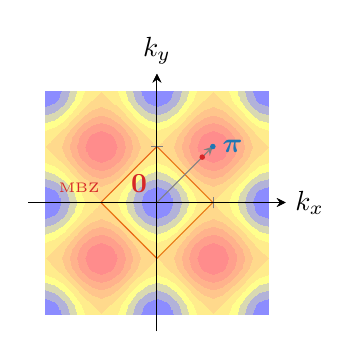
\begin{tikzpicture}
	\begin{axis}[
			axis x line=center,
			axis y line=center,
			axis z line=none,
			xmin=-2.3, xmax=2.3,
			ymin=-2.3, ymax=2.3,
			zmin=-2.5, zmax=2.5,
			xtick={1},
			ytick={1},
			xticklabel={$\pi$},
			yticklabel={$\pi$},
			xlabel={$k_x$},
			ylabel={$k_y$},
			xlabel style={anchor=west},
			ylabel style={anchor=south},
			view/az=0,
			view/el=90,
			width=0.4\textwidth,
			height=0.4\textwidth
		]
		\addplot3[
			domain=-1:0,
			color=tabred,
			dashed,
		]
		(
			{x},
			{-1-x},
			{0}
		);
		\addplot3[
			domain=0:1,
			color=tabred,
			dashed,
		]
		(
			{x},
			{-1+x},
			{0}
		);
		\addplot3[
			domain=-1:0,
			color=tabred,
			dashed,
		]
		(
			{x},
			{1+x},
			{0}
		);
		\addplot3[
			domain=0:1,
			color=tabred,
			dashed,
		]
		(
			{x},
			{1-x},
			{0}
		);
		
		\addplot3[
			domain=-2:2,
			samples=25,
			smooth,
			contour filled={number=10},
			fill opacity=0.45,
		] { -cos(deg(pi*x))-cos(deg(pi*y)) };
		
		\node[color=tabred, anchor=south east, xshift=0.3em]
			at (-1,0,0)
				{\tiny $\mathrm{MBZ}$};
		
		\draw[color=gray, -stealth]
			(0,0,0) -- (1,1,0);
		
		\fill[color=tabred]
			(0,0,0) circle (0pt) node[anchor=south east]
				{$\mathbf{0}$};
		
		\fill[color=tabblue]
			(1,1,0) circle (1pt) node[anchor=west]
				{$\bm{\pi}$};
		
	\end{axis}

	% Fine tuned
	\fill[color=tabred]
		(2.21,2.21) circle (1pt);
	
\end{tikzpicture}
		\label{appsubfig:ferromagnetic-contour}
	}
	\caption{Alternative depiction of the Hubbard square lattice hopping band previously reported in Fig.~\ref{appfig:ferromagnetic-3d-band}. The Magnetic Brillouin Zone ($\mathrm{MBZ}$) is delimited by the zero-energy contour and is indicated in figure. As it is evident, energy sign flips by taking a $(\pi,\pi)$ translation in $\mathbf{k}$ space.}
	\label{appfig:alternative-ferromagnetic-band}
\end{figure}

Consider the band of Fig.~\ref{appfig:ferromagnetic-3d-band} at half-filling. As does \citeauthor{fabrizio2022course} \cite{fabrizio2022course}, the area delimited externally by the solid lines at zero energy is denominated ``Magnetic Brillouin Zone'' ($\mathrm{MBZ}$). The periodicity of $\mathbf{k}$ space guarantees that the full $\mathrm{BZ}$ can be taken as well to be the one of Fig.~\ref{appsubfig:alternative-ferromagnetic-3d-band}. Then:
\[
\begin{aligned}
	\sum_{\mathbf{k} \in \mathrm{BZ}}
	\hat c_{\mathbf{k}\uparrow}^\dagger \hat c_{\mathbf{k}+\bm{\pi}\uparrow} &= \sum_{\mathbf{k} \in \mathrm{MBZ}}
	\left[
		\hat c_{\mathbf{k}\uparrow}^\dagger \hat c_{\mathbf{k}+\bm{\pi}\uparrow} + \hat c_{\mathbf{k}+\bm{\pi}\uparrow}^\dagger \hat c_{\mathbf{k}+2\bm{\pi}\uparrow}
	\right] \\
	&= \sum_{\mathbf{k} \in \mathrm{MBZ}}
	\left[
		\hat c_{\mathbf{k}\uparrow}^\dagger \hat c_{\mathbf{k}+\bm{\pi}\uparrow} + \hat c_{\mathbf{k}+\bm{\pi}\uparrow}^\dagger \hat c_{\mathbf{k}\uparrow}
	\right]
\end{aligned}
\]
and the same applies for spin $\downarrow$. Periodicity by shifts $2\bm{\pi}$ has been used. Now, define the Nambu spinors:
\[
	\hat \Psi_{\mathbf{k}\sigma} \equiv \begin{bmatrix}
		\hat c_{\mathbf{k}\sigma}^\dagger \\
		\hat c_{\mathbf{k}+\bm{\pi}\sigma}^\dagger 
	\end{bmatrix}
\]
and a spin-wise gap,
\[
	\Delta_\uparrow = \Delta
	\qquad
	\Delta_\downarrow = -\Delta
\]
At fixed filling, the $U$ term is a pure energy shift, thus will be neglected. The kinetic term transforms as
\[
\begin{aligned}
	-t \sum_{\langle ij \rangle} \sum_\sigma \hat c_{i\sigma}^\dagger \hat c_{j\sigma} &= \sum_{\mathbf{k} \in \mathrm{BZ}} \sum_\sigma \epsilon_\mathbf{k}^{(0)} \hat c_{\mathbf{k}\sigma}^\dagger \hat c_{\mathbf{k}\sigma} \\ 
	&= \sum_{\mathbf{k} \in \mathrm{MBZ}} \sum_\sigma \left[
		\epsilon_\mathbf{k}^{(0)} \hat c_{\mathbf{k}\sigma}^\dagger \hat c_{\mathbf{k}\sigma}
		+ \epsilon_{\mathbf{k}+\bm{\pi}}^{(0)} \hat c_{\mathbf{k}+\bm{\pi}\sigma}^\dagger \hat c_{\mathbf{k}+\bm{\pi}\sigma}
	\right] \\
	&= \sum_{\mathbf{k} \in \mathrm{MBZ}} \sum_\sigma \epsilon_{\mathbf{k}}^{(0)}  \left[
		\hat c_{\mathbf{k}\sigma}^\dagger \hat c_{\mathbf{k}\sigma}
		- \hat c_{\mathbf{k}+\bm{\pi}\sigma}^\dagger \hat c_{\mathbf{k}+\bm{\pi}\sigma}
	\right] \\ 
\end{aligned}
\]
In the second passage, the sum over the full $\mathrm{BZ}$ was written considering that the entirety of the zone is given by all the points in the $\mathrm{MBZ}$ plus their conjugates obtained by a $\bm{\pi}$ shift in the flipped band. As depicted in Fig.~\ref{appsubfig:alternative-ferromagnetic-3d-band}, kinetic energy is anti-periodic in $\mathbf{k}$ space by a vector $\bm{\pi}$. This anti-periodicity accounts for the minus sign arising in the third passage. The hamiltonian is then given by:
\[
	\hat H = \sum_{\mathbf{k} \in \mathrm{MBZ}} \sum_\sigma \hat \Psi_{\mathbf{k}\sigma}^\dagger \hat h_{\mathbf{k}\sigma} \hat \Psi_{\mathbf{k}\sigma}
	\qq{being}
	\hat h_{\mathbf{k}\sigma} \equiv \begin{bmatrix}
		\epsilon_\mathbf{k}^{(0)} & \Delta_\sigma \\
		\Delta_\sigma & - \epsilon_\mathbf{k}^{(0)}
	\end{bmatrix}
\]
Notice: the Nambu hamiltonian is a $2\times2$ matrix over the $\mathrm{MBZ}$ -- which is half the full $\mathrm{BZ}$, coherently with a solution which essentially bipartites the lattice giving back a double sized unit cell.

The system ground-state \todo

\printbibliography \nocite{*}

\end{document}
